\section{Propositional Resolution Proofs}
\label{sec:resolution}

Resolution is among the most prominent formal calculi for automated deduction and goes back to Robinson \cite{Robinson1965}.
Propositional resolution can be seen as a simplification of first-order logic resolution to propositional logic.
For basics about propositional logic and its prominent decision problem SAT, we refer the reader to \cite{Biere2009}.
For an extensive discussion of propositional and first-order logic resolution, we refer the reader to \cite{Leitsch1997}.

\begin{definition}[Literal and Clause]

A \emph{literal} is a propositional variable or the negation of a propositional variable. 
The \emph{complement} of a literal $\ell$ is denoted $\dual{\ell}$ (i.e. for any propositional variable $p$,
$\dual{p} = \neg p$ and $\dual{\neg p} = p$). 
A \emph{clause} is a set of literals. 
$\bot$ denotes the \emph{empty clause}.

\end{definition}

A clause represents the propositional logic formula that is the disjunction of its literals.
A set of clauses represents the formula that is the conjunction of its clauses.
The propositional resolution calculus operates on propositional formulas in conjunctive normal form, which are formulas that are represented by a set of clauses.
It is usual to present proofs in this calculus as syntactic derivations and refutations, that are sequences of clauses.
However, in this work, we investigate the graph structure of proofs and therefore present proofs as graphs in the following definition.

\begin{definition}[Proof] 
\label{def:proof}
A \emph{proof} $\varphi$ is a labeled directed acyclic graph $\langle V,E,\n,\mathcal{L} \rangle$, such that $\n$ has no incoming edges.
The labeling function $\mathcal{L}$ maps nodes to clauses.
The designated node $\n \in V$ is the \emph{root} of the graph, i.e. it is a node without children and every node of the graph is a recursive ancestor of the node.
Furthermore, a proof has to fulfill one of the following properties:

\begin{enumerate}
	\item $V = \{\n\}, E = \emptyset$
	\item \label{enum:resCase} 
		There are proofs $\varphi_L = \langle V_L, E_L, \n_L,\mathcal{L}_1 \rangle$ and $\varphi_R = \langle V_R, E_R, \n_R, \mathcal{L}_2 \rangle$ such that 
		$\n \notin (V_L \cup V_R)$, $\mathcal{L}_1(x) = \mathcal{L}_2(x)$ for every $x \in (V_L \cap V_R)$,
		$\mathcal{L}(\n)$ is the resolvent of $\mathcal{L}(\n_L)$ and $\mathcal{L}(\n_R)$ w.r.t. some literal $\ell$,
		for $x \in V_L: \mathcal{L}(x) = \mathcal{L}_1(x)$ and for $x \in V_R: \mathcal{L}(x) = \mathcal{L}_2(x)$,
		$V = (V_L \cup V_R) \cup \{\n \}$, $E = E_L \cup E_R \cup \{(\n_L,\n) , (\n_R,\n) \}$.
\end{enumerate}

$\mathcal{L}(\n)$ is the \emph{conclusion} of $\n$.
In case \ref{enum:resCase}, $\varphi_L$ and $\varphi_R$ are \emph{premises} of $\varphi$ and $\varphi$ is a \emph{child} of $\varphi_L$ and $\varphi_R$.
A proof $\psi$ is a \emph{subproof} of a proof $\varphi$, if they are related in the transitive closure of the premise relation.
A subproof $\psi$ of $\varphi$ which has no premises is an \emph{axiom} of $\varphi$.
$\Axioms{\varphi}$ denotes the set of nodes and axioms of $\varphi$. 
$\Premises{\n}{\varphi}$ denotes the premises and $\Children{\n}{\varphi}$ the children of the subproof with root $\n$ in a proof $\varphi$.

\end{definition}

Note that since the labeling of premises must agree on common nodes and edges, the definition of the labeling $\mathcal{L}$ is unambiguous.
Also note that in case \ref{enum:resCase} of Definition \ref{def:proof} $V_L$ and $V_R$ are not required to be disjoint. 
Therefore the underlying structure of a proof is really a directed acyclic graph and not simply a tree. 
Modern SAT- and SMT-solvers, using techniques of conflict driven clause learning, produce proofs with a  DAG structure \cite{Bouton2009,Biere2009}.
The reuse of proof nodes plays a central role in proof compression \cite{Fontaine2011}.

Several measures can be defined on proofs.
The relevant measure for this work is space, which is defined in Section \ref{sec:pebbling-game}.
Other common measures of proofs that are not discussed in this work are for example length, height, width and size of the unsat core.


\begin{example}

Consider the propositional logic formula $\Phi$ in conjunctive normal form.
$$\Phi := (x_1 \vee x_2 \vee \neg x_3) \wedge (x_1 \vee x_2) \wedge (x_1 \vee x_3) \wedge (\neg x_1)$$
In clause notation, this formula is written as $\langle \{x_1, x_2, \neg x_3\}, \{x_1, x_2\}, \{x_1, x_3\}, \{\neg x_1\} \rangle$.
By resolving the clauses $\{x_1, x_2, \neg x_3\}$ and $\{x_1, x_2\}$, we obtain the clause $\{x_1,\neg x_3\}$, which we can resolve with $\{x_1, x_3\}$ to obtain $\{x_1\}$.
Finally, we obtain the empty clause $\bot$ by resolving $\{x_1\}$ with $\{\neg x_1\}$.
The resulting proof is displayed in Figure \ref{fig:resolutionexample}.

\begin{figure}[!h]

\centering
\begin{tikzpicture}[node distance=1.5cm]

	\rootnode;
	
	\withchildren{root} {nx1}{$\{\neg x_1\}$} {x1}{$\{x_1\}$};
	\withchildren{x1}{n3}{$\{x_1,\neg x_3\}$} {n4} {$\{x_1, x_3\}$};
	\withchildren{n3}{n1}{$\{x_1,\neg x_2,\neg x_3\}$} {n4} {$\{x_1, x_2\}$};

\end{tikzpicture}

\caption{Proof of $\Phi$'s unsatisfiability}
\label{fig:resolutionexample}
\end{figure}

%\begin{figure}[!h]

%\centering
\begin{tikzpicture}[node distance=1.5cm]

	\rootnode;
	
	\proofnode[above right of=root]{ghost}{};
	\proofnode[above left of=root]{n6}{$\{x_3\}$};
	\proofnode[above right of=ghost]{n8}{$\{\neg x_3\}$};
	\drawchildren{root}{n6}{n8};
	\withchildren{n6}{n3}{$\{\neg x_2,x_3\}$} {n5} {$\{x_2\}$};
	\withchildren{n3}{n1}{$\{x_1,\neg x_2,\neg x_3\}$} {n2} {$\{\neg x_1\}$};
	\proofnode[above right of=n5]{n4} {$\{x_1,x_2\}$};
	\drawchildren{n5}{n2}{n4};
	
	\proofnode[above right of=n8]{n7} {$\{x_1,\neg x_3\}$};
	\drawchildren{n8}{n7}{n2};
	
\end{tikzpicture}

%\caption{Another Proof of $\Phi$'s unsatisfiability}
%\label{fig:resolutionexample2}
%\end{figure}

\end{example}

The aim of this work is to make proof processing easier by minimizing proofs in the two measures space and length.
Proof processing could be checking its correctness, manipulating it, as we do in this work extensively, or extracting information, for example interpolants and unsat cores, from it.
The following definition makes the notion of proof processing formal.

\begin{definition}[Proof Processing]
\label{def:proof-processing}

Let $\varphi = \langle V,E,\n,\mathcal{L} \rangle$ be a proof and $T$ be an arbitrary set.
A function $f: V \times T \times T \rightarrow T$ is a \emph{processing function} if there is a function $g_f: V \rightarrow T$ such that for every $v \in V$ with $\Premises{v}{\varphi} = \emptyset$ (i.e. $v$ represents an axiom), $g_f(v) = f(v,t_1,t_2)$ for all $\{t_1,t_2\} \subseteq T$.
Let $\mathcal{F}$ be the set of processing functions.
The \emph{apply function} $\ap: V \times \mathcal{F} \rightarrow T$ is defined recursively as follows.
$$
\ap(\n,f) = \Big\{
\begin{array}{ll}
	f(\n,\ap(pr_1,f),\ap(pr_2,f)) &\text{ if } \n \text{ has premises } pr_1 \text{ and } pr_2\\
	g_f(\n) &\text{ otherwise}\\
\end{array}
$$

\emph{Processing a node} $\n$ with some processing function $f$ means computing the value $\ap(\n,f)$.
\emph{Processing a proof} means to process its root node.

\end{definition}

\begin{example}

Checking the correctness of a proof (i.e. checking for the absence of faulty resolution steps) can be done in terms of the following processing function with $T = \{\top,\bot\}$ and $\wedge$ being the usual boolean and-operation.
$$
f(\n,w_1,w_2) = \left\{
\begin{array}{ll}
	\top & \text{ if $\n$ has no premises} \\
	w_1 \wedge w_2 &\text{ if the conclusion of $\n$ is a resolvent}\\
								 &\hspace{0.85em} \text{ of the conclusions of its premises} \\
	\bot & \text{ otherwise}
\end{array}
\right.
$$
Processing a proof with processing function $f$ yields $\top$ if and only if the proof is a correct resolution proof.
\end{example}